\chapter{L'algoritmo \emph{collapsed cone} e la sua implementazione nel TPS RayStation}
\setcounter{minitocdepth}{1}
\minitoc
\setcounter{minitocdepth}{2}
\textsf{In questo capitolo verrà descritto l'algoritmo di calcolo dosimetrico \textit{collapsed-cone-convolution} e la sua implementazione all'interno del sistema di elaborazione di piani di trattamento o treatment planning system (TPS) \RS. Ci si soffermerà in particolare sugli aspetti riguardanti le approssimazioni intrinseche dell'algoritmo assieme alle approssimazioni adottate in fase di implementazione nel TPS. Ciò è propedeutico alla comprensione dei limiti e delle precisioni raggiungibili durante la modellizzazione di un fascio clinico per trattamenti radioterapici che verrà discusso nei capitoli successivi.}

\section{La dose assorbita in radioterapia}
\label{sec:intro}
In radioterapia la \textit{dose assorbita} è quella quantità che viene utilizzata al pari della dose farmacologica per ottenere un determinato effetto terapeutico. Più precisamente, la definizione formale è fornita nel report ICRU n.85 \cite{ICRU85} come rapporto tra l'energia media $\de \bar{\varepsilon}$ impartita da radiazioni ionizzanti ad una massa $\de m$:
\begin{equation}
D = \frac{\de \bar{\varepsilon}}{\de m} \qquad\qquad \text{Unità: J\,kg}^{-1} \equiv \text{Gray [Gy]}
\end{equation} 
Esistono varie modalità di impartire una certa dose ad un paziente in radioterapia. Nell'ambito di questo lavoro si considererà solo la tecnica che fa impiego di fotoni generati da un acceleratore lineare (LINAC) denominata \virg{radioterapia a fasci esterni}.

Un LINAC è un'apparecchiatura in grado di accelerare elettroni fino ad energie dell'ordine dei 20 MeV che vanno a collidere su un target da cui si origina radiazione di frenamento (bremsstrahlung). Il fascio di fotoni così generato viene opportunamente filtrato e collimato per generare un fascio terapeutico. 
\begin{figure}
\centering
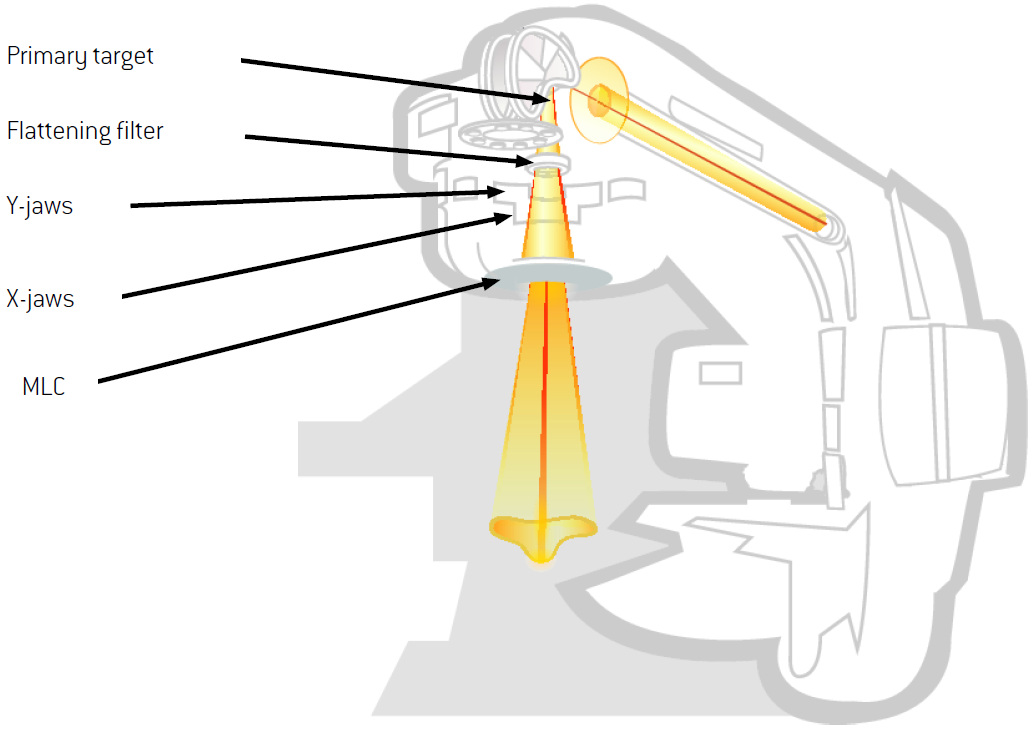
\includegraphics[width=.7\textwidth]{./cap1/linac.png}
\caption{Figura schematica di un acceleratore lineare per radioterapia a fasci esterni.}
\label{fig:linac}
\end{figure}
Tutto ciò si realizza nella testata del LINAC mediante l'uso di opportuni materiali schermanti che sono indicati nel disegno schematico riportato in Fig.\ref{fig:linac}.

 \`{E} importante notare che una parte non trascurabile di processi che vanno ad influenzare il fascio che effettivamente giunge al paziente avviene a livello della testata. Ad esempio, uno degli effetti più clinicamente rilevanti è la generazione di elettroni che \textquotedblleft contaminano\textquotedblright{} il fascio fotonico.

Una volta che il fascio clinico investe il paziente, il meccanismo di deposizione della dose è un processo molto complesso dovuto alla grande quantità di fenomeni che vengono innescati in cascata.

\begin{figure}
\centering
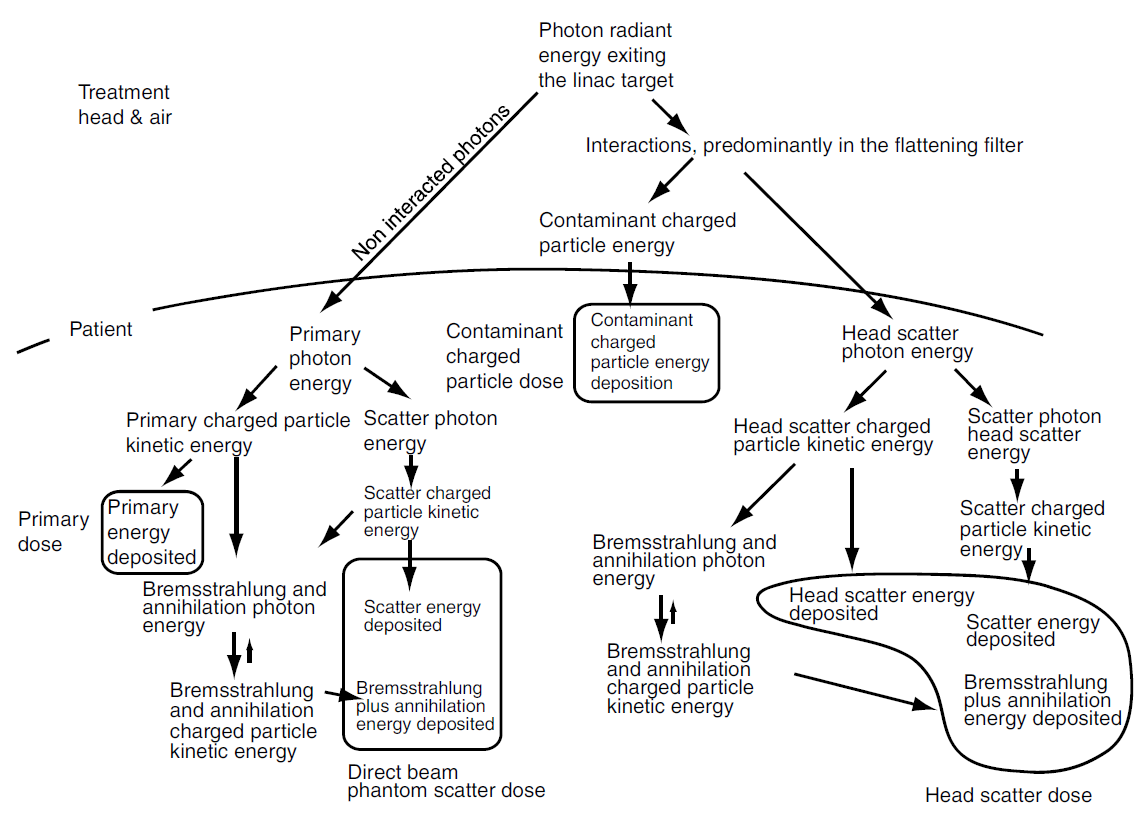
\includegraphics[width=.9\textwidth]{./cap1/processes.png}
\caption{Rappresentazione schematica delle principali interazioni che portano alla deposizione della dose nel paziente.}
\label{fig:processes}
\end{figure}
\vspace{.2cm}
La Fig.\ref{fig:processes} riassume schematicamente le principali interazioni che portano alla deposizione della dose nel paziente. \`{E} possibile identificare quattro principali meccanismi di rilascio della dose (evidenziati nella figura) che vengono elencati di seguito:
\begin{enumerate}
\item La dose primaria che rappresenta generalmente fino al 70\% della dose totale. Questa dose è generata dalla parte di fascio fotonico che non ha subito trasformazioni nella testata e che mette in moto particelle cariche le quali direttamente rilasciano la loro energia cinetica nella materia.
\item La dose di scatter dovuta alla testata (\textit{head scatter dose}) che rappresenta generalmente il 5-10\% della dose totale. Questa parte della dose è dovuta alla componente di fascio fotonico che ha subito interazioni nella testata (prevalentemente nel \textit{flattening-filter}\footnote{\label{foot:flatt} Il \textit{flattening-filter} è un dispositivo di forma piramidale che serve ad attenuare il fascio al centro in modo da realizzare una fluenza di fotoni uniforme lungo la direzione perpendicolare alla direzione di propagazione del fascio.}) e presenta una distribuzione spaziale ed energetica differente dal fascio primario. Il meccanismo di rilascio dell'energia è analogo a quello del fascio primario.
\item La dose di scatter dovuta al paziente (\textit{phantom scatter dose}) che può rappresentare fino al 30\% della dose totale. Questa componente è dovuta a tutti i processi di scatter che si innescano nel paziente a partire dal fascio primario come ad esempio fotoni di bremsstrahlung o fotoni scatterati per effetto Compton che portano ad una ionizzazione della materia con lo stesso meccanismo del fascio primario (messa in moto di elettroni).
\item La dose dovuta alle particelle di contaminazione del fascio fotonico (elettroni). Queste particelle vengono prodotte nella testata del linac sia a partire dal target (assieme ai fotoni primari) sia dall'interazione dei fotoni primari stessi con il flattening-filter. Queste particelle hanno un effetto dosimetrico rilevante (comparabile con il fascio primario) soltanto nei primi centimetri di tessuto. Questa zona è conosciuta come \textit{regione di accrescimento della dose o di build-up} della dose.
\end{enumerate}


\section{Generalità sugli algoritmi di calcolo della dose al paziente per fasci di fotoni}
Un algoritmo di calcolo dosimetrico ha lo scopo di predire gli effetti di interazione radiazione-materia con un determinato livello di accuratezza. In particolare, il fine ultimo è predire la distribuzione di dose totale assorbita nel paziente che costituisce l'entità correlata all'effetto terapeutico sul tumore o al danno sul tessuto sano. La possibilità di prevedere questa quantità è propedeutica al processo noto come \textit{pianificazione del trattamento} in cui vengono adoperate delle opportune scelte riguardanti la collimazione e l'intensità del fascio volte a minimizzare il rapporto rischio/beneficio della terapia.

Esistono due grandi classi di algoritmi dosimetrici:
\begin{itemize}
\item Algoritmi \textit{correction-based}.
\item Algoritmi \textit{model-based}.
\end{itemize}
Gli algoritmi correction-based sono algoritmi empirici. Essi sono  basati su un gruppo di dati misurati in certe condizioni di riferimento e fanno uso di fattori o funzioni matematiche di tipo analitico o di tipo look-up-table per predire la distribuzione di dose assorbita in altre condizioni. 
Questi metodi furono i primi ad essere implementati in quanto non necessitano di grosse potenze di calcolo ma, d'altro canto, presentano dei limiti di accuratezza intrinseci per situazioni complesse (mezzi non omogenei, interfacce tra tessuti, campi di irradiazione molto irregolari o ad intensità modulata\ldots). Un'estensiva review di questi tipi di algoritmi è stata pubblicata da Fraass \textit{et al.}\cite{Fraass1995}.

\vspace{.2cm}
L'avvento della rivoluzione tecnologica e la crescita della potenza di calcolo disponibile, ha permesso l'implementazione degli algoritmi model-based i quali simulano i processi di interazione radiazione-materia  a partire da principi primi tramite un modello fisico-matematico.\\
In questo caso il set di misure iniziali è unicamente utilizzato per ottimizzare i parametri del modello che poi viene applicato per predire la distribuzione di dose assorbita nei vari scenari clinici. Questi algoritmi hanno dimostrato una maggiore accuratezza rispetto ai correction-based ed al giorno d'oggi i più utilizzati sono quelli basati su metodi semi-analitici (algoritmi di convolution/superposition) oppure algoritmi statistici basati su metodo Monte Carlo.

Il TPS RayStation in particolare implementa un algoritmo di tipo convolution/superposition conosciuto come \textit{collapsed cone convolution} sviluppato, a partire dalla metà dagli anni '80, indipendentemente da Mackie e Ahnesj{\"{o} \cite{Ahnesjo1989, Boyer1998, Mackie1985, Ahnesjo1987}.



\section{La sovrapposizione e la convoluzione in termini matematici}
Le operazioni di sovrapposizione e di convoluzione sono concetti matematici largamente utilizzati in fisica. Ragionando unicamente in termini matematici, l'operazione di sovrapposizione consiste nella combinazione lineare di una serie di funzioni $f_i(x)$, ognuna con un proprio peso $c_i$:
\begin{equation}
g(x) = \sum_{i=1}^{N} c_i\cdot f_i(x)
\end{equation}
Un tipico esempio fisico dell'operazione di sovrapposizione è il calcolo del campo elettrico in un punto dovuto ad una certa distribuzione di cariche puntiformi:
\begin{equation}
\mathbf E_0(\mathbf r) = \sum_{i=1}^N \mathbf E_{0i}(r) = \frac {1}{4 \pi \varepsilon_0} \sum_{i=1}^N q_i \frac {\mathbf r - \mathbf r_i'} {\left \| \mathbf r - \mathbf r_i' \right \|^3}
\end{equation}
Nel caso continuo, l'operazione di sovrapposizione può essere espressa con un integrale, esteso a tutto il dominio di definizione del problema, tra una funzione primaria $p$ ed una funzione coefficiente $s$ come funzione kernel:
\begin{equation}
\label{eq:sovrapp_math}
D(x,y,z) = \int_V p(x',y',z')\, s(x,x',y,y',z,z')\de x' \de y' \de z'
\end{equation}
Un particolare caso dell'operazione di sovrapposizione è rappresentato dalla convoluzione che si realizza quando la funzione kernel è spazialmente invariante, ovvero dipende solo dalla differenza tra la coordinata $(x,y,z)$ e la variabile di integrazione $(x',y',z')$:
\begin{equation}
\label{eq:convol_math}
D(x,y,z) = \int_V p(x',y',z')\, s(x-x',y-y',z-z')\de x' \de y' \de z'
\end{equation}


\section{Il calcolo della dose come sovrapposizione di eventi}
\label{sec:teoria_conv}
Il problema del calcolo della dose in un punto all'interno di un volume è in generale un problema di sovrapposizione di eventi che può essere tradotto matematicamente con l'Eq.\eqref{eq:sovrapp_math}.
\begin{figure}
\centering
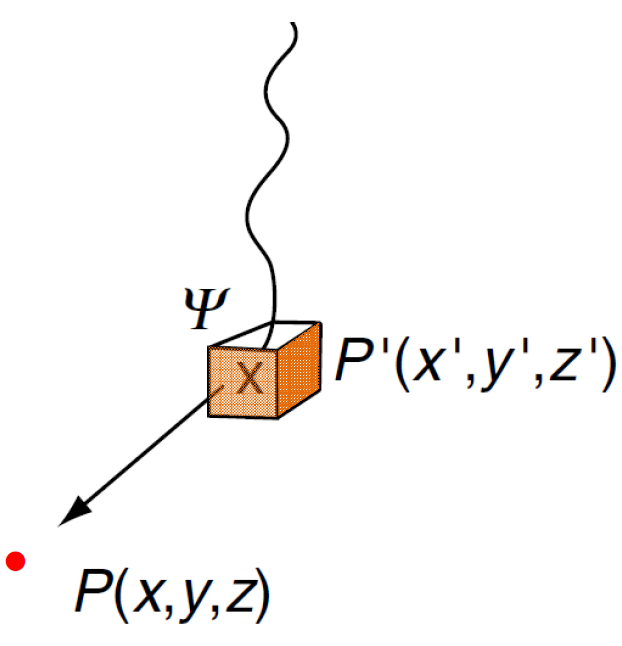
\includegraphics[width=.45\textwidth]{./cap1/superp1.png}
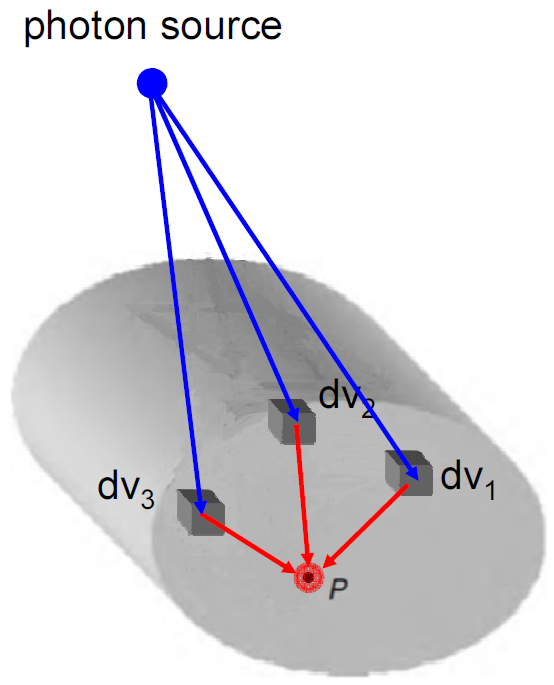
\includegraphics[width=.45\textwidth]{./cap1/superp2.png}
\caption{Il calcolo della dose visto come sovrapposizione di eventi.}
\label{fig:superp}
\end{figure}

Nello specifico, osservando la Fig.\ref{fig:superp}, si nota come la quantità di energia che viene assorbita in un punto $P$ dipenda da infiniti contributi dovuti alle particelle ionizzanti messe in moto dai fotoni nei loro rispettivi centri di interazione $P'$.\\
La distribuzione dell'energia rilasciata dai fotoni nei centri di interazione primaria $P'$ va a formare una quantità denominata TERMA (total-energy-released-in-matter).  \\
Il TERMA è esprimibile come il prodotto tra la \textit{fluenza di energia primaria} (quantità di energia radiante incidente per unità di superficie [J m$^{-2}$]) e il coefficiente di assorbimento lineare massico del mezzo $(\mu/\rho)$ \cite{Ahnesjo1987}.

Introducendo la funzione di scatter\footnote{Funzione conosciuta anche come \textit{energy deposition point kernel} o \textit{point spread kernel} o \textit{kernel di deposizione}.} $s(x'\rightarrow x, y'\rightarrow y, z'\rightarrow z)$ che esprime l'ammontare di energia assorbita nel punto $P(x,y,z)$ dovuta all'energia rilasciata nell'interazione avvenuta nel punto $P'(x',y',z')$, la dose assorbita nel punto $P$ è esprimibile con un integrale:
\begin{align}
D(x,y,z) &=  \int_V \frac{\mu}{\rho} \Psi(x',y',z')\,s(x'\rightarrow x, y'\rightarrow y, z'\rightarrow z)\, \de x' \de y' \de z'\\
         &= \int_V T(x',y',z')\,s(x'\rightarrow x, y'\rightarrow y, z'\rightarrow z)\, \de x' \de y' \de z'\\
         &= \int_V T(P')\,s(P'\rightarrow P)\, \de V'
\end{align}

Questa equazione è valida nel caso di un fascio di fotoni monoenergetico in un mezzo omogeneo di densità $\rho$. La generalizzazione al caso polienergetico si effettua introducendo il TERMA differenziale in energia $T(P',E)$ e la funzione di scatter polienergetica $s(P'\rightarrow P,E)$ ed integrando su tutte le energie coinvolte:
\begin{equation}
D(P) = \iint_{E,V} T(P',E)\,s(P'\rightarrow P,E)\, \de V' \de E
\label{eq:superp}
\end{equation}
L'equazione \eqref{eq:superp} matematicamente è un'operazione di sovrapposizione, così come espresso nell'Eq.\eqref{eq:sovrapp_math} e rispecchia il fatto per cui la dose calcolata in un punto $P$ è la sovrapposizione di tanti fenomeni che avvengono nei punti $P'$. In aggiunta, considerando il caso di un mezzo omogeneo ed infinitamente esteso, la funzione di scatter risulta spazialmente invariante per cui l'\eqref{eq:superp} è un'equazione di convoluzione del tipo indicato nella \eqref{eq:convol_math}. Questa condizione matematica rispecchia il fenomeno fisico cosiddetto dell'\textit{equilibrio di particelle cariche}\footnote{L'equilibrio di particelle cariche (CPE) sussiste all'interno di un volume qualora il numero di particelle ionizzanti che entrano in esso, è uguale al numero di particelle che ne fuoriesce.}.

%Verrà dimostrato nelle sezioni successive come l'Eq.\eqref{eq:superp} possa essere scritta nella forma:
%\begin{equation}
%\boxed{D(\vec{r}) = \iint_{E,V} T_E(\rho_{\vec{r'}} \cdot \vec{r})\, s_E(\rho_{\vec{r}-\vec{r'}}\cdot (\vec{r}-\vec{r'}))\de\vec{r'} \de E}
%\label{eq:superp_true}
%\end{equation}
%che rappresenta la cosiddetta \textit{equazione di convolution/superposition} per il calcolo della dose in un volume disomogeneo investito da un fascio di fotoni polienergetico.



\section{Il calcolo della dose in RayStation}
\label{sec:algo_Ray}
Il calcolo della dose nel TPS RayStation fa uso del formalismo illustrato nelle sezioni precedenti e procede in quattro principali passaggi:
\begin{enumerate}
\item Il calcolo della fluenza di energia.
\item Il calcolo del TERMA.
\item L'applicazione delle opportune funzioni di scatter e del principio di \textit{convolution-superposition} per il calcolo della dose finale.
\item La somma del contributo dovuto alle particelle di contaminazione (elettroni).
\end{enumerate}

\subsection{Il calcolo della fluenza di energia}
\label{sec:fluence}
Questo primo step consiste in un calcolo geometrico che non tiene conto della presenza del paziente. Si è già notato nella sezione introduttiva (Fig.\ref{fig:processes}) come il fascio in ingresso in un paziente sia costituito da una parte primaria e da una parte che ha interagito con gli elementi della testata (in particolare con il flattening-filter). RayStation tratta queste due componenti con un modello a due sorgenti poste ad una certa distanza lungo la direzione di propagazione del fascio (Fig.\ref{fig:twosources}a).
\begin{figure}
\centering
a)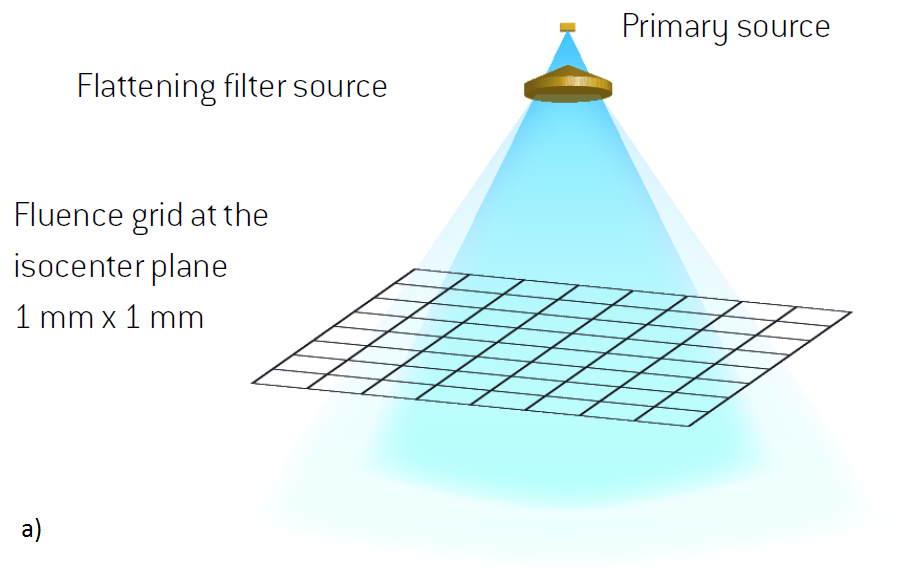
\includegraphics[width=.5\textwidth]{./cap1/twosources.png}
b)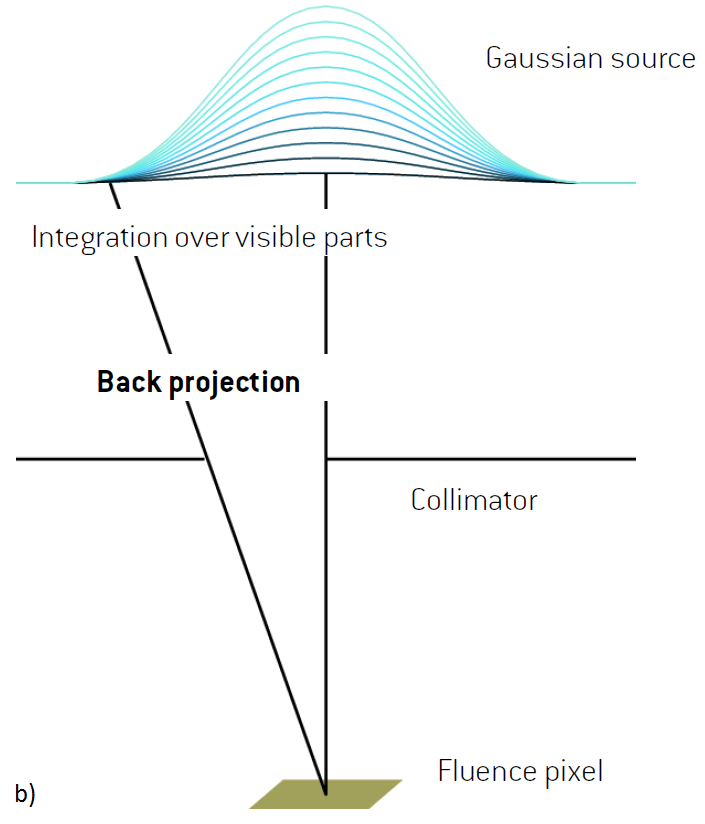
\includegraphics[width=.4\textwidth]{./cap1/source_int.png}
\caption{(a) modello a due sorgenti utilizzato per il calcolo della fluenza di energia. (b) processo di integrazione della parte visibile della sorgente per il calcolo della fluenza.}
\label{fig:twosources}
\end{figure}
La sorgente primaria è modellizzata con un profilo gaussiano ellittico esteso dell'ordine dei mm mentre la sorgente di scatter del flattening-filter è gaussiana circolare estesa dell'ordine dei centimetri \cite{Chaney1994}.\\
Il calcolo della fluenza viene effettuato su un piano passante per il centro di simmetria rotazionale del LINAC denominato \textit{isocentro} e perpendicolare alla direzione del fascio (Fig.\ref{fig:twosources}a).
Le sorgenti vengono geometricamente proiettate attraverso i collimatori indicati in Fig.\ref{fig:linac} costituiti da blocchi di materiale schermante (\textit{jaws}) e da un dispositivo fatto di lamelle retraibili (\textit{multi-leaf-collimator}) che serve a generare conformazioni irregolari del fascio.\\
Matematicamente, l'operazione di calcolo della fluenza consiste in un'integrazione pixel per pixel della parte di sorgente \textquotedblleft visibile\textquotedblright{} attraverso i collimatori (Fig.\ref{fig:twosources}b) con un metodo di backprojection.\\
La mappa di fluenza così ottenuta viene corretta per includere alcuni fenomeni come la trasmissione dei collimatori, la trasmissione della punta e del bordo delle lamelle (\textit{leaf tip e tongue}\&\textit{groove}), il peso relativo delle sorgenti ed altri processi che verrano discussi in seguito.

In parallelo viene computata la mappa di fluenza per le sorgenti di elettroni di contaminazione (generati secondo le modalità descritte nella Sez.\ref{sec:intro}). Queste ultime sono gaussiane circolari e poste alla stessa posizione delle sorgenti di fotoni. Esse sono divise in primaria e di scatter del flattening filter e la loro intensità è espressa in percentuale rispetto alla fluenza dei fotoni primari.

\subsection{Il calcolo del TERMA}
Il TERMA costituisce la prima parte dell'integrale per il calcolo della dose assorbita (Eq.\ref{eq:superp}). Esso quantifica l'assorbimento della fluenza di energia che attraversa il paziente. A partire da questo assorbimento vengono applicate le funzioni di scatter per generare la distribuzione di dose.\\
Il TERMA differenziale in energia può essere scritto nella seguente forma generale:
\begin{equation}
\label{eq:termaE}
T(\vec{r'},E) = \frac{\mu}{\rho}(\vec{r'},E)\,\Psi(\vec{r'},E)
\end{equation}
dove $\vec{r'}$ è la coordinata del punto di interazione primaria, $\mu/\rho$ il coefficiente di assorbimento lineare massico, $\Psi$ la fluenza di energia primaria ed $E$ l'energia del fascio primario.

\begin{figure}
\centering
a)\includegraphics[width=.45\textwidth]{./cap1/TERMA_isoPlane.eps} b)
\includegraphics[width=.45\textwidth]{./cap1/TERMA_isoPatient.eps}
\caption{(a) calcolo della fluenza sul piano isocentrico senza considerare il paziente. (b) proiezione della fluenza sul piano parallelo al piano isocentrico e corrispondente alla superficie del paziente (ad una distanza sorgente-superficie del paziente (SSD).}
\label{fig:terma}
\end{figure}
Il paziente è modellizzato all'interno del TPS tramite uno studio di tomografia computerizzata che contiene una mappa di densità dei tessuti. Questo permette di conoscere il primo termine dell'Eq.\eqref{eq:termaE} \cite{RaySearchLaboratories2014}.\\
Il calcolo del secondo termine della \eqref{eq:termaE} avviene seguendo questi passaggi:
\begin{itemize}
\item Si parte dalla mappa di fluenza calcolata sul piano passante per l'isocentro e perpendicolare alla direzione di propagazione del fascio senza considerare la presenza del paziente (Fig.\ref{fig:terma}a).
\item La mappa di fluenza calcolata in assenza del paziente viene proiettata e riscalata verso la sorgente fino ad una distanza pari a $\vec{r_0}$ ove $\vec{r_0}$ costituisce la distanza dalla sorgente primaria alla superficie del paziente (distanza nota come Source-Surface-Distance o SSD) (Fig.\ref{fig:terma}b).
\item La mappa di fluenza calcolata all'ingresso del paziente $\Psi(\vec{r_0},E)$ viene rimodulata all'interno di questi (studio CT) tenendo conto di due fenomeni:
\begin{itemize}
\item L'assorbimento della radiazione di tipo esponenziale con il coefficiente di assorbimento (nota anche come legge di Lambert-Beer): $\exp{\left( -\int_{\vec{r_0}}^{\vec{r'}} \mu(\vec{r'},E) \de l \right)}$.
\item La divergenza del fascio che da luogo ad una decrescita della fluenza con l'inverso del quadrato della distanza ($|\vec{r_0}|^2 / |\vec{r'}|^2$).
\end{itemize}
\end{itemize}
L'equazione che si ottiene per la fluenza riferita ad un qualsiasi punto di coordinata $\vec{r'}$ all'interno del paziente è:
\begin{equation}
\label{eq:fluence}
\Psi(\vec{r'},E) = \frac{|\vec{r_0}|^2}{|\vec{r'}|^2}\Psi(\vec{r_0},E)\,\exp{\left( -\int_{\vec{r_0}}^{\vec{r'}} \mu(\vec{r'},E) \de l \right)}
\end{equation}
Lo studio CT del paziente viene discretizzato nel TPS su una griglia di voxel cubici detta \textit{dose grid} (su cui poi verrà calcolata la distribuzione di dose). I voxel della dose-grid campionano le densità fornite dalla CT da cui viene ricavato il coefficiente di assorbimento locale $\mu / \rho(\vec{r'},E)$.\\
Moltiplicando il termine $\mu / \rho(\vec{r'},E)$  con la fluenza espressa dalla \eqref{eq:fluence} si ottiene la distribuzione di TERMA all'interno del paziente (Eq.\eqref{eq:termaE}).



\subsection{Applicazione delle funzioni di scatter}
\label{sec:scatter_fun}

\begin{figure}
\centering
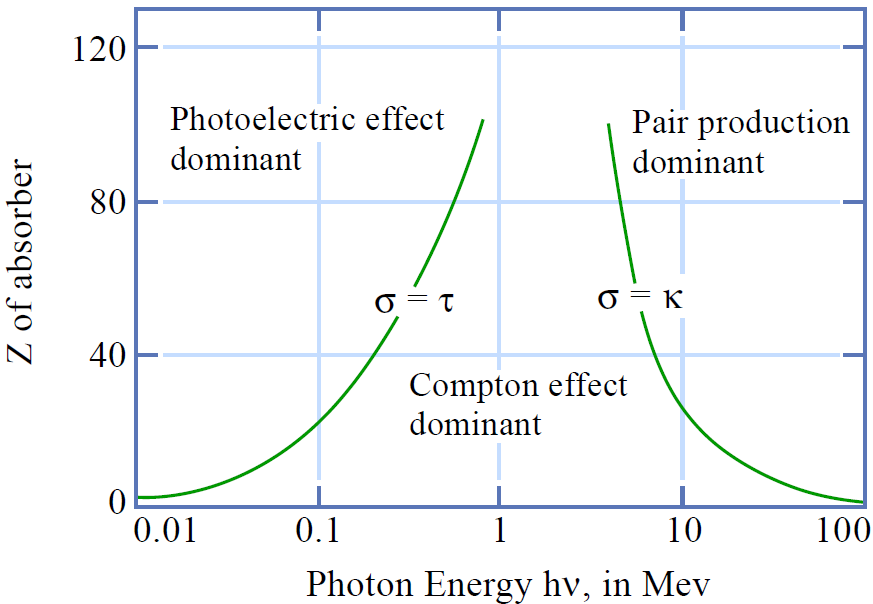
\includegraphics[width=.7\textwidth]{./cap1/compt_dom.png}
\caption{Prevalenza degli effetti di interazione dei fotoni con la materia in funzione dell'energia del fotone. L'effetto Compton è prevalente per le energie e i materiali tipici della radioterapia.}
\label{fig:compt_dom}
\end{figure}
Alle energie tipiche dei fotoni utilizzati in radioterapia l'effetto predominante è l'effetto Compton (Fig.\ref{fig:compt_dom}) secondo cui l'interazione del fotone primario genera un fotone diffuso ed un elettrone con una certa energia cinetica. Una modellizzazione completa del trasporto del fotone diffuso e dell'elettrone messo in moto richiede un approccio statistico di tipo Monte Carlo, computazionalmente molto dispendioso. L'approccio convolution/superposition racchiude i processi statistici di deposizione dell'energia nella funzione di scatter introdotta nell'Eq.\eqref{eq:superp} ed agisce in maniera deterministica.

La funzione di scatter è ottenibile a partire da una simulazione Monte Carlo in cui un unico fotone viene fatto interagire forzatamente all'interno di un volume omogeneo di acqua (elemento più simile ai tessuti molli umani) e si va ad osservare la deposizione della dose che ne deriva. Questa operazione è stata effettuata da Mackie \cite{Mackie1985} utilizzando il software Monte Carlo EGS sviluppato dallo Stanford Linear Accelerator Center che pubblicò nella metà degli anni '80 delle funzioni di scatter discretizzate in forma tabulare (vedi Fig.\ref{fig:mackie_kernels}).
\begin{figure}
\centering
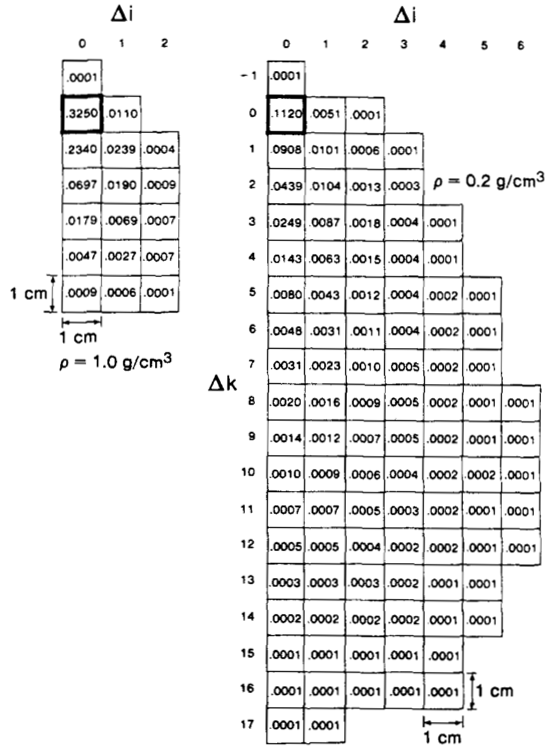
\includegraphics[width=.8\textwidth]{./cap1/mackie_kernels.png}
\caption{Funzione di scatter calcolate per un fotone da 15MV e per due differenti materiali di densità  1g/cc (acqua) e 0.2g/cc. \cite{Mackie1985}}
\label{fig:mackie_kernels}
\end{figure}

Nota la funzione di scatter, assieme alla distribuzione di TERMA, è necessario procedere alla risoluzione dell'integrale indicato nell'Eq.\eqref{eq:superp} per arrivare alla distribuzione di dose assorbita. 
Questa operazione è effettuata per via numerica (tramite computer) e presuppone una discretizzazione dello spazio di integrazione e delle funzioni integrande. I metodi adottabili sono i seguenti:\\

\textbf{Somma diretta:\\}
Applicando le funzioni di scatter (kernel) ai punti di deposizione del TERMA, in linea di principio è possibile arrivare alla dose assorbita in maniera triviale risolvendo per somma diretta l'integrale \eqref{eq:superp}. Tuttavia, questa operazione su una griglia di $N^3$ voxel e generalizzata ad un mezzo disomogeneo, risulta essere un problema  di ordine $N^7$ \cite{Ahnesjo1989}. Un tale numero di operazioni è difficilmente gestibile anche con le moderne potenze di calcolo\footnote{Se immaginiamo di discretizzare un paziente di dimensioni $20x20x20$ cm$^3$ con voxel di lato $0.3$ cm otteniamo una griglia di circa $70x70x70$ voxel. Il numero di operazioni da effettuare risolvendo numericamente l'integrale \eqref{eq:superp} sarebbe $70^7\approx 10^{13}$. Disponendo di un computer capace di effettuare operazioni con frequenza dell'ordine del GHz$\equiv 10^9\,s^{-1}$ il tempo di risolvere $10^{13}$ operazioni sarebbe $t=10^{13}/10^9\,s=10^5\,s\approx 2\, ore!$.}. \\

\textbf{Metodo di Fast Fourier Transform (FFT):\\}
Un possibile approccio alternativo alla risoluzione della \eqref{eq:superp} si basa sulla considerazione per cui, nel caso di un mezzo omogeneo, la funzione di scatter della \eqref{eq:superp} risulta essere spazialmente invariante (l'integrale è un prodotto di convoluzione). Questo permette l'applicazione della teoria degli spazi di Fourier per cui l'integrale di convoluzione  diventa un semplice prodotto delle trasformate delle funzioni nello spazio di Fourier. L'operazione di antitrasformata del prodotto delle funzioni trasformate permette di ottenere la distribuzione di dose. Questa operazione è stata dimostrata comportare un numero di operazioni inferiore alla somma diretta pari a $N^3\log_2 N$ \cite{Wong1996}. Il limite di questa metodologia è che risulta esattamente applicabile solo su uno spazio continuo. La discretizzazione che inevitabilmente va effettuata per un calcolo numerico comporta delle approssimazioni. Inoltre questo metodo risulta essere difficilmente estensibile al caso disomogeneo in cui il kernel perde di invarianza spaziale. Sono stati studiati vari approcci basati su correzioni orientate a recuperare l'invarianza spaziale dei kernel anche nel caso disomogeneo. I risultati tuttavia non si sono rivelati soddisfacenti se comparati con il metodo presentato nel paragrafo successivo \cite{Wong1996}.\\

\textbf{Metodo di \textit{Collapsed-cone-convolution}:\\}
Questo metodo è quello che si è rivelato il più soddisfacente nella storia degli algoritmi \textit{model-based} in quanto facilmente estensibile al caso disomogeneo e polienergetico. Contiene inoltre come parte fondante una discretizzazione spaziale dei kernel di deposizione facilmente adattabile ad un calcolo numerico tramite computer. Il metodo \textit{collapsed-cone} è alla base del motore dosimetrico implementato nel TPS RayStation e verrà presentato nel dettaglio nella sezione successiva.


\subsection{L'approssimazione \textit{collapsed-cone}}
L'algoritmo collapsed-cone discretizza spazialmente i kernel di deposizione prima di effettuare la convoluzione in modo da tener conto del trasporto della radiazione non in tutte le direzioni ma solo in un loro sottoinsieme (questa operazione avverrebbe in ogni caso impiegando un qualsiasi metodo di risoluzione numerico tramite computer).

Questo approccio è stato presentato indipendemente da Mackie \cite{Reckwerdt1992} e Ahnesj\"{o} \cite{Ahnesjo1989} e fu denominato \textit{collapsed-cone}. Il confronto della dose ottenuta con questo metodo ed il metodo Monte Carlo fornì risultati eccellenti per l'epoca. Questi risultati rappresentano ancora oggi il benchmark per il calcolo della dose con TPS utilizzando metodi non statistici.
\begin{figure}[!t]
\centering
a) 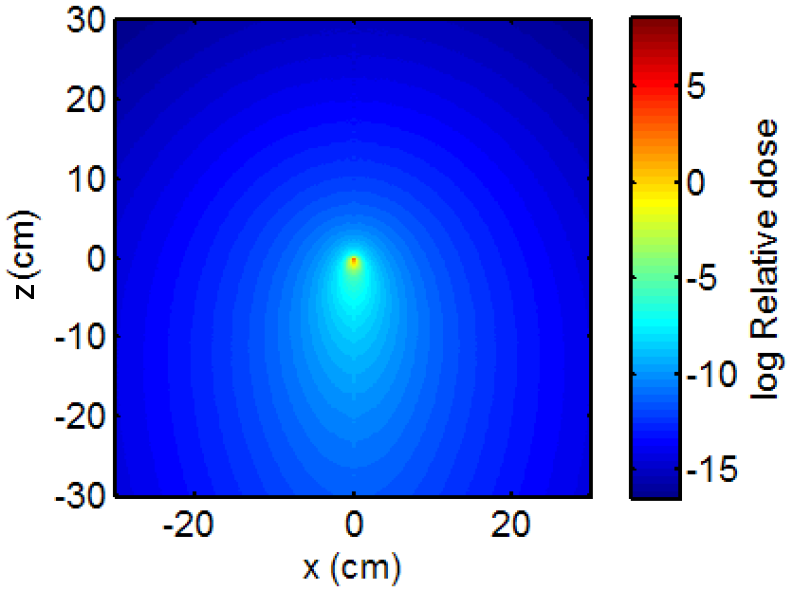
\includegraphics[width=.42\textwidth]{./cap1/kern_ray1.png}$\quad$
b) 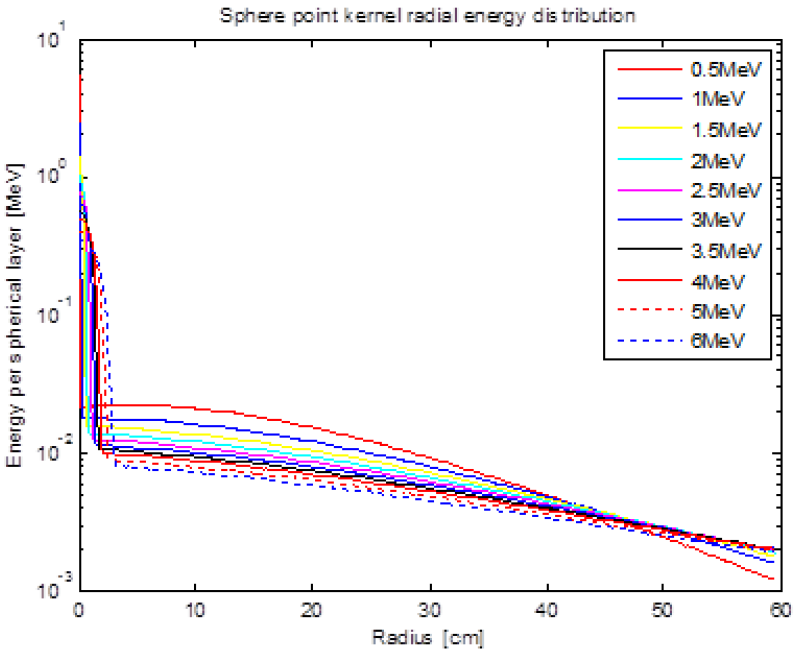
\includegraphics[width=.42\textwidth]{./cap1/kern_ray2.png}
\caption{(a) distribuzione planare di un kernel di deposizione. (b) distribuzione 1D di alcuni kernel al variare dell'energia; da notare una prima parte di rilascio rapido di energia dovuta agli elettroni Compton ed una parte più estesa dovuta ai fotoni secondari diffusi che a loro volta re-interagiscono con il mezzo.}
\label{fig:kern_ray}
\end{figure}

Per capire il meccanismo alla base di questa approssimazione partiamo con l'osservare in Fig.\ref{fig:kern_ray} la distribuzione spaziale tipica di alcuni kernel di deposizione. La discretizzazione di questi kernel può essere effettuata in maniera diretta lungo delle semplici linee di integrazione seguendo un processo noto come \textit{ray-tracing}.
\begin{figure}
\centering
a)\includegraphics[width=.4\textwidth]{./cap1/Kernel_RayTr.eps}
b)\includegraphics[width=.45\textwidth]{./cap1/Kernel_CCC.eps}
\caption{(a) Errore di sampling che si commette discretizzando il kernel solo lungo dei raggi (Ray-tracing). (b) Meccanismo di ridistribuzione della dose in un settore conico sul proprio asse (Collapsed-cone).}
\label{fig:raytrace_vs_cc}
\end{figure}
Tuttavia Ahnesj\"{o} notò che questo metodo di discretizzazione semplicistico può portare ad un errore di sampling ampio a causa sia della divergenza dei raggi di ray-tracing sia della particolare forma dei kernel di deposizione  \cite{Ahnesjo1989} (i.e. una larga parte di deposizione di energia non viene conteggiata a meno di usare un campionamento angolare fittissimo complicato da gestire a livello computazionale (vedi Fig.\ref{fig:raytrace_vs_cc}a)).\\
Per questo Ahnesj\"{o} propose di discretizzare i kernel in coordinate sferiche con dei coni aventi il vertice nel punto di interazione e sottendenti un certo angolo solido. Tutte le deposizioni di energia contenute all'interno della superficie conica che sottende l'angolo solido vengono \textquotedblleft\textit{collassate}\textquotedblright{} sull'asse del cono stesso (vedi Fig.\ref{fig:raytrace_vs_cc}b). Con questa procedura, l'energia totale depositata risulta spazialmente ridistribuita ma viene conteggiata per intero.

L'operazione di \textquotedblleft\textit{collassamento}\textquotedblright{} dei kernel avviene matematicamente come segue. In primo luogo si effettua un fit analitico del kernel di deposizione calcolato tramite metodologie Monte Carlo. La funzione proposta da Ahnesj\"{o} per questo scopo in coordinate sferiche ha la seguente forma:
\begin{equation}
\label{eq:kern_fit}
s(r,\theta) = \frac{A_\theta e^{-a_\theta r} + B_\theta e^{-b_\theta r}}{r^2}
\end{equation}
dove $A_\theta,\,a_\theta,\,B_\theta$ e $b_\theta$ sono parametri di fit che dipendono dall'angolo di scatter $\theta$. I due termini esponenziali descrivono l'uno la caduta rapida del kernel dovuto agli elettroni Compton primari e l'altro la coda più lenta dovuta alle interazioni di scatter secondarie (Fig.\ref{fig:kern_ray}b). Da notare che il kernel possiede una simmetria cilindrica per cui l'angolo $\phi$ della tripletta di coordinate sferiche ($r,\theta,\phi$) non è esplicitato. La validità di questo fit è mostrata in Fig.\ref{fig:kern_fit}.
\begin{figure}
\centering
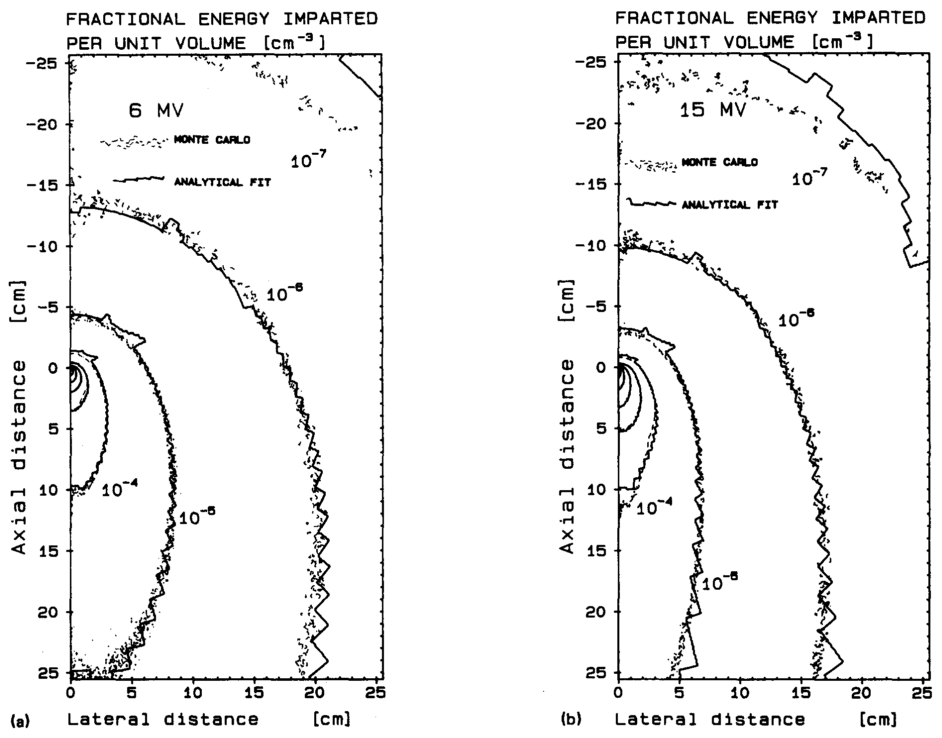
\includegraphics[width=.8\textwidth]{./cap1/kern_fit.png}
\caption{Fit analitico dei kernel di deposizione per un fotone da 6MV (a) e da 15MV (b) \cite{Ahnesjo1989}.}
\label{fig:kern_fit}
\end{figure}

Stabilendo un angolo solido $\Omega_i$, l'operazione di \virg{collassamento} è un'integrazione in coordinate sferiche del kernel espresso dalla \eqref{eq:kern_fit} (vedi anche Fig.\ref{fig:kern_collaps}):
\begin{equation}
\iint_{\Omega_i} s(r,\theta) r^2\de \Omega_i = A_{\Omega_i} e^{-a_{\Omega_i} r} + B_{\Omega_i} e^{-b_{\Omega_i} r} \equiv K(r,\Omega_i)
\end{equation}
La funzione $K(r,\Omega_i)$ è quella da convolvere con la mappa del TERMA per arrivare alla mappa di dose assorbita.

Il metodo collapsed-cone esteso al caso più generico (fascio polienergetico e mezzo disomogeneo) è stato dimostrato comportare un numero di operazioni dell'ordine di $MN^3$ dove $M$ è il numero di settori in cui viene diviso l'angolo solido ed $N$ è il numero di voxel della griglia di dose/TERMA \cite{Ahnesjo1989}. Questo risultato è da confrontare con l'ordine $N^7$ in caso di somma diretta di tutti i termini che si ottengono discretizzando l'integrale \eqref{eq:superp} oppure con $N^3\log_2N$ nel caso di applicazione del metodo di trasformata di Fourier.

\begin{figure}
\centering
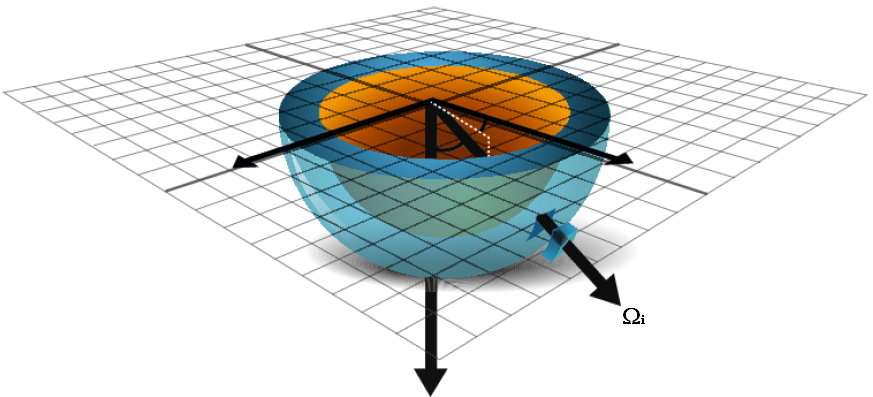
\includegraphics[width=\textwidth]{./cap1/kern_collaps.png}
\caption{Operazione di \textit{collapsing} dei kernel all'interno di segmenti conici definiti dall'angolo solido $\Omega_i$.}
\label{fig:kern_collaps}
\end{figure}

In RayStation il numero di settori in cui viene discretizzato il kernel è 128 che corrisponde a 8 direzioni lungo l'angolo di scatter $\theta$ e 16 lungo l'angolo di simmetria cilindrica $\phi$. Il campionamento è più fitto nella direzione di propagazione del fascio dove è presente il gradiente più intenso.

Così come implementato il metodo non richiede nelle ipotesi che il kernel sia un invariante spaziale come nel caso del metodo a trasformata di Fourier. Questo rende semplice dal punto di vista computazionale  la generalizzazione al caso disomogeneo che verrà trattata in seguito alla generalizzazione al caso polienergetico nelle sezioni a seguire.

\begin{figure}
\centering
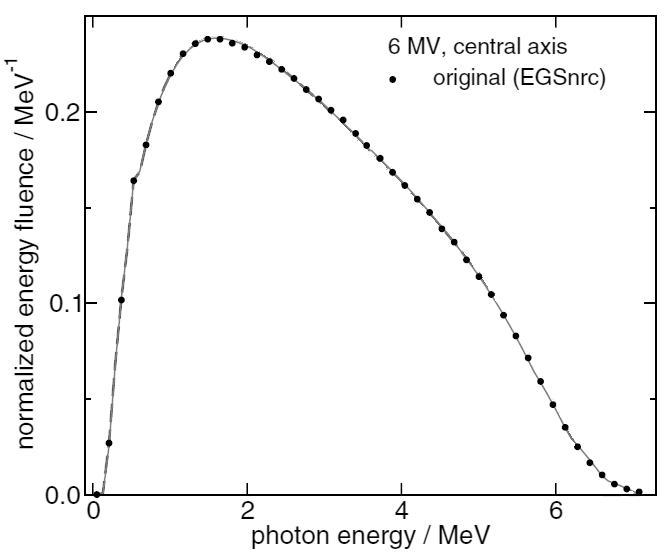
\includegraphics[width=.7\textwidth]{./cap1/LinacSpectrum.png}
\caption{Spettro di energia tipico di un fascio radioterapico di energia 6MV (solo componente fotonica)}
\label{fig:LinacSpectrum}
\end{figure}

\subsection{La generalizzazione al caso polienergetico}
Un tipico fascio di fotoni generato da un LINAC per radioterapia contiene uno spettro polienergetico (vedi Fig.\ref{fig:LinacSpectrum}). Inoltre lo spettro subisce uno spostamento verso energie più alte a causa dell'attraversamento della materia (effetto di \textit{depth-hardening}). Questo suggerisce il fatto che non è possibile considerare un unico kernel di deposizione nel passaggio dal TERMA alla dose. Boyer et al. assieme a Zhu e Van Dyk \cite{Boyer1989,Zhu1995} hanno dimostrato che una discretizzazione in 5 bin sia sufficiente a rappresentare lo spettro di un LINAC da 6MV. Sulla base di ciò, Papanikolaou et al. \cite{Papanikolaou1993} hanno investigato i possibili metodi di estensione del metodo convolution al caso polienergetico dimostrando che è sufficiente combinare kernel monoergetici pesati con le relative componenti spettrali. Nel medesimo lavoro viene dimostrato che il problema del depth-hardening può essere risolto riscalando i kernel con dei fattori che dipendono dalla lunghezza radiologica attraversata.

Per applicare questi principi, nel TPS sono memorizzati una serie di point spread kernel computati con il motore Monte Carlo EDKnrc incluso in EGS4nrc per le seguenti energie del fotone primario incidente: 0.5, 1, 1.5, 2, 2.5, 3, 3.5, 4, 5, 6, 7, 8, 9 10, 12, 14, 16, 18, 20 MeV. Queste energie corrispondono ai bin implementati in RayStation per rappresentare uno spettro fotonico (es. per un fascio da 6 MV i bin coinvolti vanno da 0.5 a 6 MV).\\
Ad ogni bin dello spettro corrisponde un singolo kernel monoenergetico. Il kernel polienergetico viene calcolato mediante media dei singoli kernel monoenergetici pesati con l'intensità delle rispettive componenti spettrali  \cite{Papanikolaou1993}. Questo processo è raffigurato schematicamente nella Fig.\ref{fig:kern_trans}a.
In seguito viene costruita una libreria di 600 kernel riscalati su un ampio intervallo di lunghezze radiologiche per tenere conto dell'effetto di \textit{depth-hardening} nelle varie situazioni cliniche.


\subsection{La generalizzazione al caso disomogeneo}

Considerando un mezzo con varie disomogeneità, la funzione di scatter perde la sua invarianza spaziale per cui l'equazione \eqref{eq:superp} cessa di essere un'integrale di convoluzione. In termini fisici, in un mezzo disomogeneo non sussiste più l'equilibrio di particelle cariche in ogni punto del volume.

In condizioni standard i kernel sono calcolati in un volume omogeneo di acqua, tuttavia la deposizione di energia cambia se i processi di ionizzazione avvengono in un mezzo differente. Per questo motivo, in linea di principio, i kernel di deposizione andrebbero di volta in volta ricalcolati a seconda della situazione.\\
Mackie propose un'approssimazione orientata ad evitare di ricalcolare i kernel in ogni singola situazione clinica. Secondo questa approssimazione, il kernel di deposizione per un mezzo disomogeneo si può ottenere a partire dal kernel calcolato in acqua e sostituendo tutte le lunghezze fisiche ($l$) con le lunghezze radiologiche ($\rho_{H_2O}^{e^-}\cdot\,l$) (dove $\rho_{H_2O}^{e^-}$ è la densità elettronica del mezzo relativa alla densità elettronica dell'acqua\footnote{\`E necessario utilizzare la densità elettronica in quanto è tra gli elettroni del mezzo che avvengono le interazioni che portano all'assorbimento della dose.}) \cite{Mackie1985}. Questa operazione è nota con il nome di \textit{density-scaling} dei kernel di deposizione ed era in realtà conosciuta già prima dell'avvento degli algoritmi di convolution come Teorema di O'Connor \cite{OConnor1957}.\\
\begin{figure}[!t]
\centering
a) 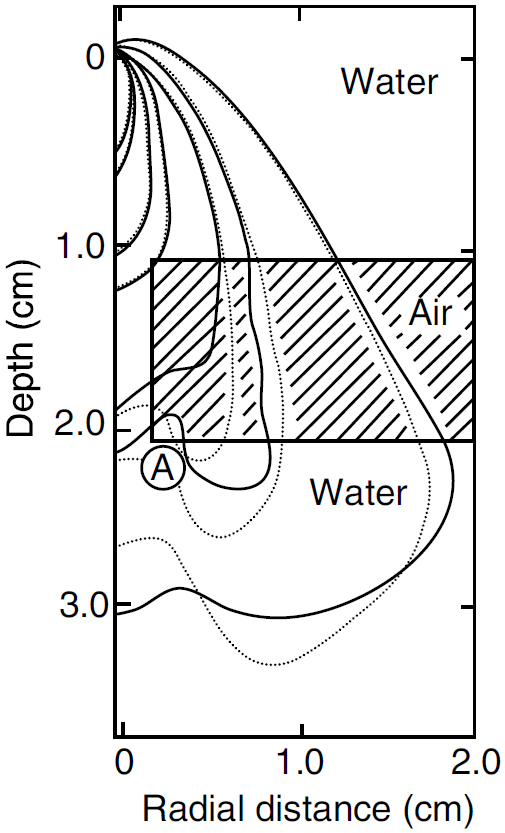
\includegraphics[width=.36\textwidth]{./cap1/kern_dens.png}
b)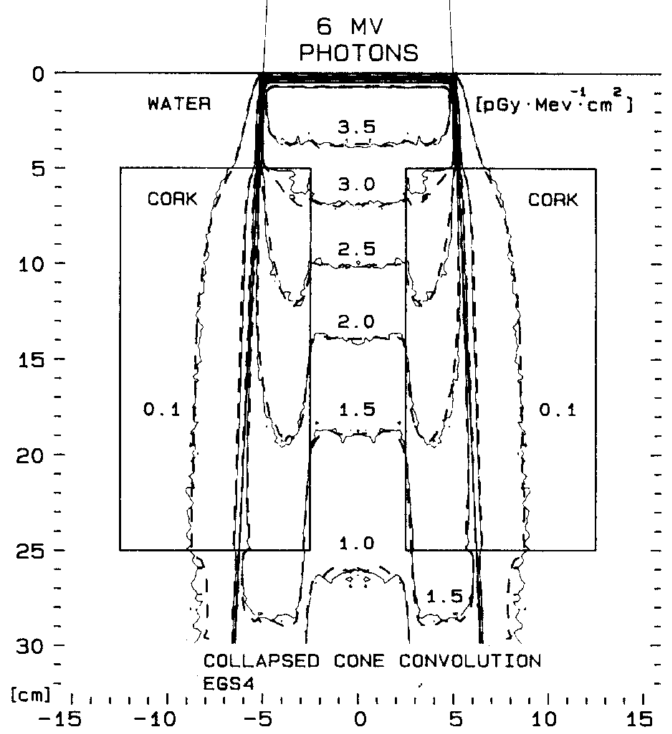
\includegraphics[width=.5\textwidth]{./cap1/kern_dens2.png}
\caption{(a) Confronto tra un kernel calcolato direttamente con un metodo Monte Carlo (linea solida) e un kernel calcolato in condizioni omogenee riscalato secondo la lunghezza radiologica (linea tratteggiata); le isolinee corrispondono ad una dose relativa di 1000, 500, 100, 50, 10, 5, 1; il punto A posizionato appena sotto l'interfaccia aria/acqua presenta la massima discrepanza (50\%). (b) effetto globale su un insieme di interazioni; un \textit{averaging} delle incertezze sui singoli kernel si risolve in un accordo accettabile su un fantoccio complesso che simula un torace \cite{Woo1990,Arnfield2000,Ahnesjo1989}.}
\label{fig:kern_dens}
\end{figure}
In particolare questo teorema fu formulato per mettere in relazione la dose calcolata in due mezzi di differente densità ma stessa composizione chimica. In queste condizioni O'Connor dimostrò che il numero di fotoni scatterati rispetto al numero di fotoni primari rimane invariato nei due mezzi qualora tutte le distanze geometriche (includendo anche la dimensione del campo, la distanza dalla sorgente etc.) siano riscalate con le lunghezze radiologiche \cite{OConnor1957}. Le ipotesi alla base di questo teorema sono:
\begin{itemize}
\item Mezzo infinitamente esteso (per cui si realizza la condizione di equilibrio di particelle cariche).
\item Composizione chimica dei due mezzi identica.
\end{itemize}
Queste condizioni non sono realizzabili in pratica per cui è inevitabile che il metodo del density-scaling dei kernel comporti degli errori quando applicato ad una situazione clinica reale.

Nella Fig.\ref{fig:kern_dens}a si può notare l'errore che si commette applicando il teorema di O'Connor nella forma suggerita da Mackie ai kernel di deposizione in una configurazione di disomogeneità aria/acqua che può simulare una situazione tessuto/polmone (Woo e Cunningham \cite{Woo1990}). Nonostante la comparazione del kernel calcolato direttamente e del kernel calcolato con il metodo del density-scaling presenti degli errori fino al 50\%, è stato dimostrato \cite{Ahnesjo1989} che su un insieme numeroso di interazioni interviene un effetto di \textit{averaging} per cui discrepanze significative rimangono solo in condizioni di estrema disomogeneità, ossia vicino alle interfacce in cui si ha un cambio repentino di densità (vedi Fig.\ref{fig:kern_dens}b).

%L'integrale espresso nell'Eq.\ref{eq:superp} può essere riscritto per un mezzo omogeneo nella forma \cite{Khan2010}:
%\begin{equation}
%D(x,y,z) =  \int_V \frac{\mu}{\rho} \Psi(x',y',z')\,s(x'- x, y'- y, z'- z)\, \de x' \de y' \de z'
%\label{eq:superp_homo}
%\end{equation}
%Questa equazione rappresenta \textit{principio di convolution} per il calcolo della dose. Considerando un mezzo infinitamente esteso, la funzione $s$ è spazialmente invariante. Si è già accennato nella Sez.\ref{}

In Fig.\ref{fig:kern_trans}b è riportato un diagramma schematico della modificazione di un kernel in un mezzo disomogeneo quando viene applicato il metodo del \textit{density-scaling}.

Applicando il teorema del \textit{density-scaling} (o di O'Connor) alla \eqref{eq:superp}, sostituendo le lunghezze fisiche con le lunghezze radiologiche \cite{Khan2010} si ottiene la seguente equazione:
\begin{equation}
D(\vec{r}) = \iint_{E,V} T_E(\rho_{\vec{r'}} \cdot \vec{r})\, s_E(\rho_{\vec{r}-\vec{r'}}\cdot (\vec{r}-\vec{r'}))\de\vec{r'} \de E
\label{eq:superp_disom}
\end{equation}
dove $(\rho_{\vec{r'}} \cdot \vec{r})$ è la lunghezza radiologica dalla sorgente di fotoni fino al punto di interazione primaria (ove viene rilasciato il TERMA) e $\rho_{\vec{r}-\vec{r'}}\cdot (\vec{r}-\vec{r'})$ è la lunghezza radiologica dal punto di interazione primaria al punto di deposizione della dose.\\
Questa equazione è nota come equazione di \textit{convolution-superposition} e rappresenta il problema generico del calcolo della dose per un fascio polienergetico e mezzo disomogeneo. Essa è alla base del motore dosimetrico implementato in RayStation ed è risolta numericamente utilizzando il metodo collapsed-cone.

\begin{figure}
\centering
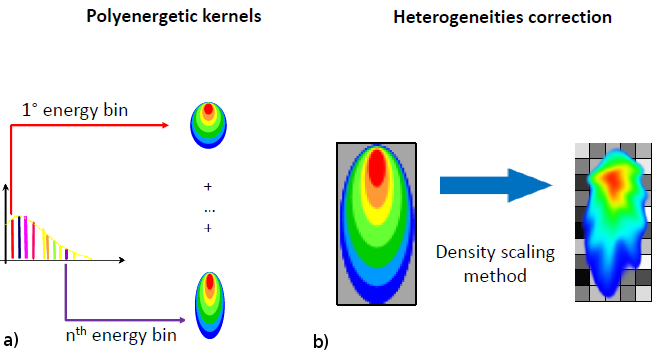
\includegraphics[width=\textwidth]{./cap1/kern_trans.png}
\caption{(a) figura schematica del metodo con cui si costruisce il kernel polienergetico (combinazione di kernel monoenergetici pesati con la componente spettrale). (b) figura schematica che rappresenta come il kernel si modifica quando viene riscalato tenendo conto delle lunghezze radiologiche attraversate nelle varie direzioni.}
\label{fig:kern_trans}
\end{figure}




\section{Approssimazioni aggiuntive}
Nella sezione precedente sono state mostrate le approssimazioni intrinseche dell'algoritmo \textit{collapsed-cone}. In questa sezione evidenziamo delle ulteriori approssimazioni adottate in RayStation orientate all'aumento della velocità di calcolo della dose.

\subsection{L'approssimazione \textit{no-kernel-tilting}}
Un fascio di fotoni generato da un LINAC è tipicamente divergente all'aumentare della distanza dalla sorgente. I kernel di deposizione dell'energia sono calcolati per un fascio che incide verticalmente ed hanno l'asse orientato nella medesima direzione. Un'applicazione rigorosa del metodo convolution/superposition richiederebbe la rotazione dei kernel per allinearli lungo l'angolo di incidenza del raggio primario (vedi Fig.\ref{fig:kern_tilt}a).\\
\begin{figure}
\centering
a)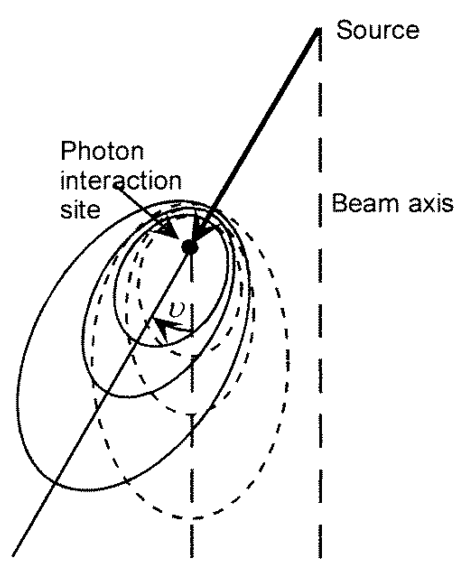
\includegraphics[width=.3\textwidth]{./cap1/kern_tilt.png}
b)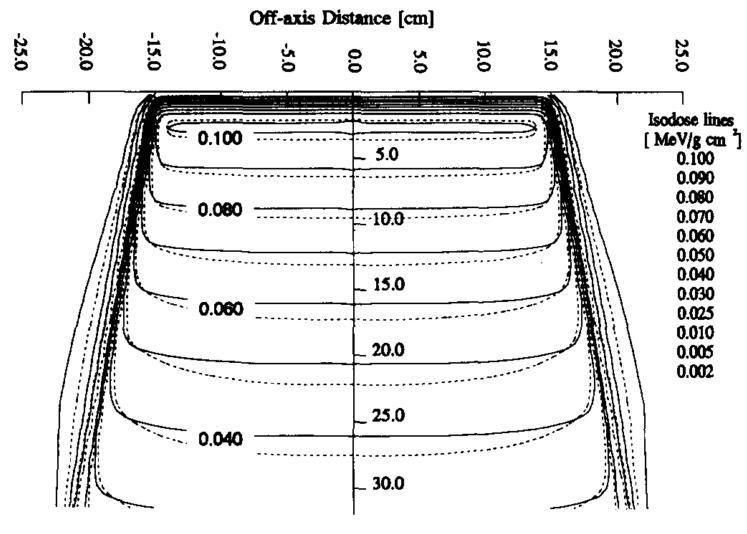
\includegraphics[width=.55\textwidth]{./cap1/kern_tilt_b.png}
\caption{(a) I kernel di deposizione dovrebbero essere ruotati dello stesso angolo di incidenza $\nu$ del raggio primario; tuttavia per ridurre considerevolmente i tempi di calcolo, si applicano kernel con orientazione verticale. (b) il non ruotare i kernel comporta una deposizione di dose maggiore verso il centro del fascio (linea tratteggiata) confrontata con la dose calcolata senza approssimazione (linea solida).}
\label{fig:kern_tilt}
\end{figure}
Questa operazione implicherebbe molteplici rotazioni di matrici \cite{Sharpe1997} con il risultato di aumentare considerevolmente il tempo di calcolo della dose. 
%Oltre a questo, un ulteriore grande vantaggio dell'approssimazione \textit{no-kernel-tilting} consiste nel fatto di poter calcolare solo una volta le intersezioni dei raggi uscenti dai kernel con la griglia di dose\footnote{Operazione nota come \textit{raytracing}.} e di riutilizzare i risultati per i voxel successivi.
Per questo motivo vari autori hanno sviluppato dei metodi che consentissero di applicare kernel di deposizione non ruotati (\textit{no-kernel-tilting}) \cite{Sharpe1997,Papanikolaou1993}.

In RayStation è implementato il metodo suggerito da Papanikolaou et al. \cite{Papanikolaou1993}. L'idea di questo metodo sta nel considerare che, non ruotando i kernel, si ha un accumulo di dose maggiore verso il centro del fascio (Fig.\ref{fig:kern_tilt}b).\\ 
Papanikolaou ha dimostrato come questo può essere recuperato con i seguenti passaggi:
\begin{enumerate}
\item Si rimuove la divergenza dalla fluenza di energia (termine $|\vec{r_0}|^2/|\vec{r'}|^2$ nell'Eq.\eqref{eq:fluence}).
\item Si applicano i point spread kernel con l'approssimazione di \textit{no-tilting}.
\item Si riapplica la divergenza riscalando la dose calcolata con il fattore $|\vec{r_0}|^2/|\vec{r}|^2$ dove $\vec{r}$ è la coordinata di calcolo della dose (diversa dalla coordinata di rilascio del TERMA $\vec{r'}$).
\end{enumerate}
L'effetto dell'operazione n.1 è quello di aumentare la fluenza di energia lontano dal centro del fascio. Applicando poi i punti 2 e 3 si arriva ad una distribuzione in cui la dose approssima quella calcolata considerando i kernel ruotati.\\
Sharpe e Papanikolaou \cite{Sharpe1997,Papanikolaou1993} hanno evidenziato come l'approssimazione di \textit{no-tilting} dei kernel presenti i suoi limiti solo in situazioni difficilmente realizzabili clinicamente. In particolare, discrepanze oltre il 3\% si osservano in caso di basse distanze sorgente-superficie del paziente (SSD $< 70$ cm) congiuntamente all'utilizzo di campi estesi ($> 20x20$ cm$^2$).

\begin{figure}
\centering
\includegraphics[width=.6\textwidth]{./cap1/TERMADepos.eps}
\caption{Distinzione delle zone utilizzate nell'approssimazione \textit{full-TERMA-deposition}. (CCC: Collapsed Cone Convolution)}
\label{fig:TERMADepos}
\end{figure}

\subsection{Approssimazioni \textit{full-TERMA-deposition} e \textit{adaptive interpolation}}
Ulteriori approssimazioni denominate \textit{full-TERMA-deposition} e \textit{adaptive interpolation} sono volte ad evitare di applicare rigorosamente il metodo di collapsed-cone-superposition su ogni voxel della griglia di dose.\\
A questo proposito, la \textit{full-TERMA-deposition} può essere riassunta in quattro principali step:
\begin{enumerate}
\item Alla fine del calcolo della distribuzione di TERMA vengono identificati quei voxel in cui è stato depositato un TERMA minore dello 0.5\% del massimo TERMA rilasciato nel volume (zona (1) nella Fig.\ref{fig:TERMADepos}).
\item A partire da questi voxel viene costruita una iso-superficie che viene poi espansa di una lunghezza radiologica di 5 cm isotropicamente.
\item All'interno del volume compreso tra la superficie TERMA$_i= 0.5\%$ TERMA$_{max}$ e la sua espansione di $5$ cm  il trasporto avviene solo su alcune delle 128 direzioni del kernel di deposizione (zona (2) nella Fig.\ref{fig:TERMADepos}). 
\item Al di fuori della superficie precedentemente calcolata non viene effettuato il trasporto del TERMA con l'algoritmo collapsed-cone bensì si assume un rilascio locale di tutta l'energia (zona (3) nella Fig.\ref{fig:TERMADepos}).
\end{enumerate}
Questa approssimazione è stata osservata generare un'errore sul calcolo della dose minore dello 0.2\% su punti in generale a bassa rilevanza clinica \cite{RaySearchLaboratories2014}.\\

\begin{figure}[!t]
\centering
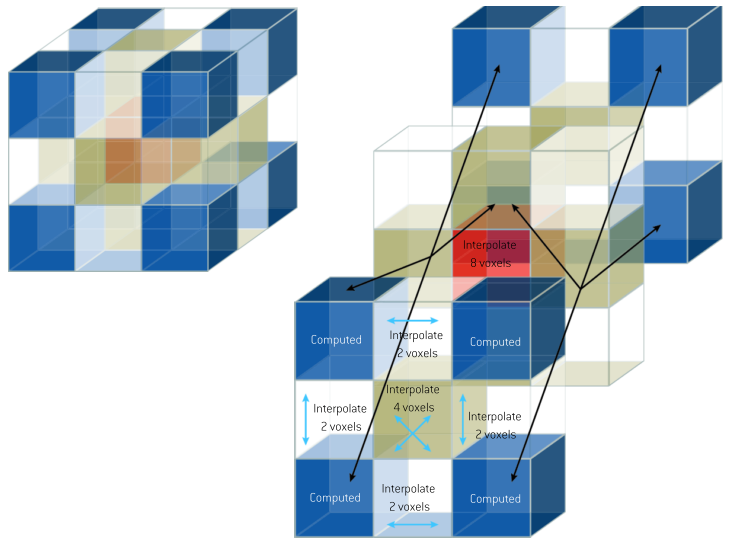
\includegraphics[width=.8\textwidth]{./cap1/dose_interp.png}
\caption{L'approssimazione di \textit{adaptive interpolation}. I voxel in blu sono quelli calcolati con l'algoritmo collapsed-cone.}
\label{fig:dose_interp}
\end{figure}

La seconda approssimazione di \textit{adaptive interpolation} si basa su un preliminare calcolo della dose su voxel alternati per identificare zone a basso od alto gradiente. Per le zone a basso gradiente la dose nei voxel non coinvolti nel computo preliminare viene calcolata con la media dei voxel adiacenti; per le zone ad alto gradiente viene applicato l'algoritmo completo. In particolare gli step che vengono seguiti sono riassumibili nei seguenti punti:
\begin{enumerate}
\item Dopo il calcolo della distribuzione di TERMA si effettua un primo calcolo della dose ogni due voxel come illustrato nella Fig.\ref{fig:dose_interp}.
\item Un voxel viene considerato appartenere ad una zona a basso gradiente se la massima differenza tra il TERMA nei voxel adiacenti è minore dello 0.2\% e la massima differenza in dose è minore del 5\% della dose massima.
\item Per i voxel appartenenti alla zona a basso gradiente la dose viene calcolata mediando i voxel adiacenti che possono essere in numero di 2, 4 o 8 a seconda della posizione (vedi Fig.\ref{fig:dose_interp}).
\item Per i voxel appartenenti alla zona ad alto gradiente viene applicato l'algoritmo completo.
\end{enumerate}
Per un semplice campo $10x10$ cm$^2$ ed energia 6 MV, la distribuzione di dose calcolata senza applicare la \textit{adaptive interpolation} si correla con la dose calcolata utilizzando l'approssimazione con un coefficiente di correlazione maggiore di 0.99999. Gli errori più rilevanti si registrano vicino alla penombra del fascio dove rimangono comunque entro il 2\% \cite{RaySearchLaboratories2014}.


\section{Dose aggiuntiva da elettroni di contaminazione}
\label{sec:dose_electr}
Come già accennato nella sezione introduttiva (Fig.\ref{fig:processes}), nei primi centimetri di tessuto una parte rilevante della dose totale è dovuta agli elettroni di contaminazione del fascio fotonico. Questi elettroni si originano prevalentemente da processi di scatter dei fotoni con i collimatori ed il flattening-filter all'interno della testata.\\
Alle energie tipiche della radioterapia, la deposizione della dose di un fascio elettronico avviene repentinamente all'aumentare della profondità (vedi Fig.\ref{fig:electr_enloss}a).
\begin{figure}
\centering
a) 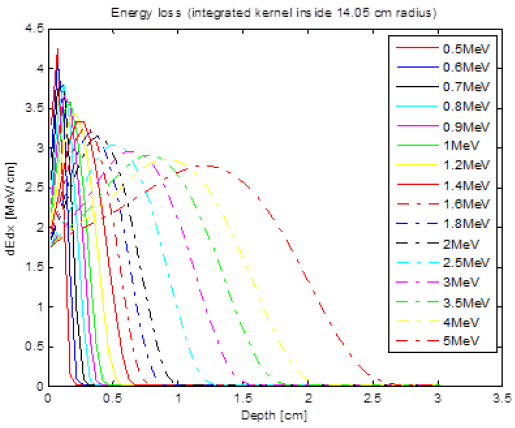
\includegraphics[width=.45\textwidth]{./cap1/electr_enloss.png}
b) 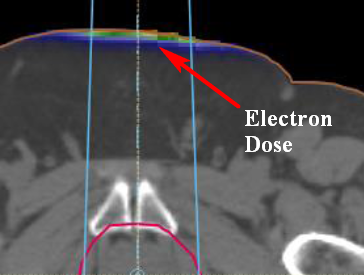
\includegraphics[width=.44\textwidth]{./cap1/electr_doseCT_zoom.png}
\caption{(a) diagrammi della dose rilasciata in funzione della profondità di un fascio di elettroni a varie energie. (b) distribuzione di dose dovuta ad elettroni di contaminazione del fascio calcolata su una CT. Da notare è che questa dose risulta importante solo nei primi millimetri di tessuto attraversato.}
\label{fig:electr_enloss}
\end{figure}

L'algoritmo dosimetrico implementato in RayStation per il calcolo della dose da contaminazione elettronica rientra nella classe degli algoritmi \textit{model-based} basati su \textit{convolution/superposition}, con una variante sul kernel di deposizione che non è più puntuale ma esteso di forma cilindrica (vedi Fig.\ref{fig:electr_pencil}). 

\begin{figure}
\centering
a) 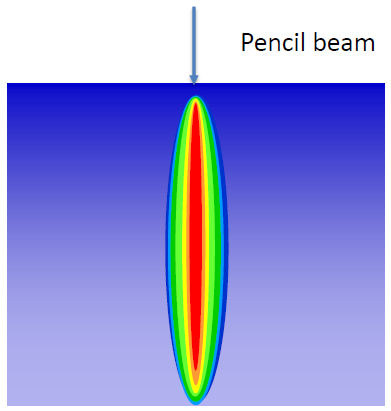
\includegraphics[width=.4\textwidth]{./cap1/electr_pencil.png}$\qquad$
b) 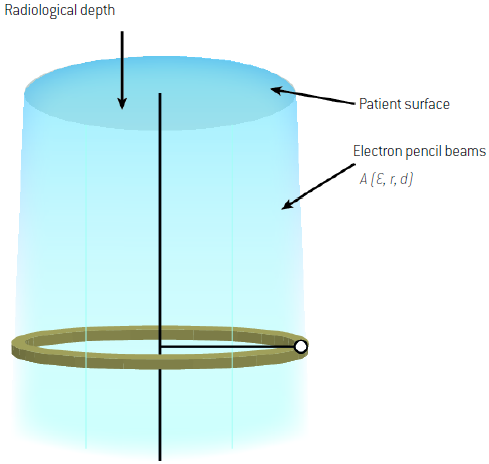
\includegraphics[width=.4\textwidth]{./cap1/electr_pencil_b.png}
\caption{(a) kernel di deposizione di tipo \textit{pencil-beam}. (b) figura schematica che mostra la simmetria cilindrica nel calcolo della dose quando si utilizza un kernel di tipo \textit{pencil-beam}.}
\label{fig:electr_pencil}
\end{figure}


Questo tipo di algoritmo è denominato \textit{pencil-beam} e rappresenta una versione semplificata del collapsed-cone.\\
L'equazione che permette il calcolo della dose è analoga alla \eqref{eq:superp} rappresentabile in coordinate cilindiriche:
\begin{equation}
\label{eq:electr_superp}
D(d) = 2\pi \iint_{E,V} \Psi(r,d,E)\, s(r,d,E)\, r\de r \de E
\end{equation}
dove $E$ e $V$ sono rispettivamente l'energia ed il volume di integrazione, $r$ la coordinata di integrazione e $d$ il punto di valutazione della dose.
L'Eq.\eqref{eq:electr_superp} è implementata all'interno di RayStation in maniera analoga al caso dei fotoni. Schematicamente i passaggi che vengono seguiti sono:
\begin{itemize}
\item I kernel \textit{pencil-beam} sono pre-calcolati con un modello Monte Carlo (software EGSnrc).
\item Viene utilizzato un modello a due sorgenti per calcolare la fluenza di energia elettronica in assenza del paziente.
\item Viene calcolata la distribuzione di TERMA utilizzando la formula della perdita di energia per ionizzazione di Bethe-Bloch per gli elettroni nella materia \cite{RaySearchLaboratories2014}.
\item Vengono applicati i kernel \textit{pencil-beam} per modellizzare lo scatter laterale degli elettroni.
\end{itemize}

Nella Fig.\ref{fig:electr_enloss}b è mostrata la distribuzione di dose dovuta agli elettroni di contaminazione calcolata su una CT di un paziente. Questa dose viene sommata alla dose dovuta ai fotoni calcolata con l'algoritmo collapsed-cone. 















